\xiti
\begin{xiaotis}

\xiaoti{求证:和三角形两边同时垂直的直线,也和第三边垂直。}

\xiaoti{求证:如果一条直线平行于一个平面,那么这个平面的任何垂线都和这条直线垂直。}

\xiaoti{直角三角形 $ABC$ 在平面 $\alpha$ 内, $D$ 是斜边 $AB$ 的中点。
    $AC = 6$ cm, $BC = 8$ cm, $EC \perp \alpha$, $EC = 12$ cm。
    求 $EA$、$EB$、$ED$的长。
}

\xiaoti{如图,钳工检查长方块工件的棱 $BB'$ 是否和底面 $A'C'$ 垂直,
    只要检查 $\angle BB'A'$ 和 $\angle BB'C'$ 是不是直角就可以了,为什么?
}

\begin{figure}[htbp]
    \centering
    \begin{minipage}[b]{7cm}
        \centering
        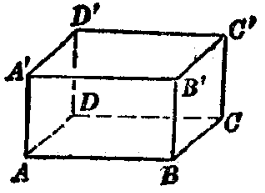
\includegraphics[width=4cm]{../pic/ltjh-ch1-xiti4-04.png}
        \caption*{(第 4 题)}
    \end{minipage}
    \qquad
    \begin{minipage}[b]{7cm}
        \centering
        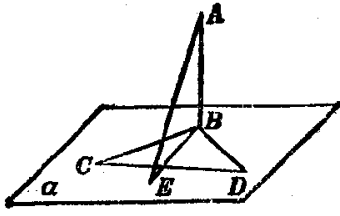
\includegraphics[width=5cm]{../pic/ltjh-ch1-xiti4-05.png}
        \caption*{(第 5 题)}
    \end{minipage}
\end{figure}

\xiaoti{如图, $AB = 5$ cm, $BC \perp AB$, $BD \perp AB$,
    在 $BC$、$BD$ 所在的平面 $\alpha$ 内有一点 $E$, $BE = 7\;\limi$。
    (1)$EB$ 和 $AB$, $CD$ 和 $AB$ 成多少度角?
    (2)$AE$ 的长是多少?
}

\xiaoti{证明:斜线上的所有的点在平面上的射影,必在同一条直线上。}

\xiaoti{有一旗竿高 8 m, 它的顶点挂一条长 10 m 的绳子,
    拉紧绳子并把它的下端放在地面上两点(和旗竿脚不在同一直线上)。
    如果这两点都和旗竿脚距离 6 m,那么旗竿就和地面垂直,为什么?
}

\xiaoti{在一个工件上同时钻很多孔时,常用多头钻,多头钻杆都是互相平行的,
    在工作时,只要调整工件表面和一个钻杆垂直,工件表面就和其他钻杆都垂直。为什么?
}

\xiaoti{已知: $\alpha \cap \beta = CD$, $EA \perp \alpha$, $EB \perp \beta$。 求证: $CD \perp AB$。}

\xiaoti{求证:两条平行线和同一个平面所成的角相等。}

\xiaoti{用反证法证明:}
\begin{xiaoxiaotis}

    \xxt{过一点和一个平面垂直的直线只有一条;}

    \xxt{过一点和一条直线垂直的平面只有一个。}

\end{xiaoxiaotis}


\xiaoti{经过一个角的顶点引这个角所在平面的斜线。如果斜线和这个角两边的夹角相等,
    那么斜线在平面上的射影是这个角的平分线所在的直线。
}

% TODO: wrapfigure 在这里无法正常使用
\begin{minipage}{10.5cm}
    \jiange

    \xiaoti{从平面外一点 $D$ 向平面引垂线段 $DA$ 及斜线段 $DB$、$DC$。
        已知:$DA = a$, $\angle BDA = \angle CDA = 60^\circ$, $\angle BDC = 90^\circ$。
        求 $BC$ 的长。
    }

    \xiaoti{有一方木料如图,上底面上有一点 $E$, 要经过点 $E$ 在上底面上画一条直线和 $C$、$E$ 的连线垂直,应怎样画?}

    \xiaoti{平面 $\alpha$ 内有一个正六边形,它的中心是 $O$, 边长是 2 cm。
        $OH \perp \alpha$, $OH = 4$ cm。 求点 $H$ 到这个正六边形顶点和边的距离。
    }

\end{minipage}
\quad
\begin{minipage}{4cm}
    \centering
    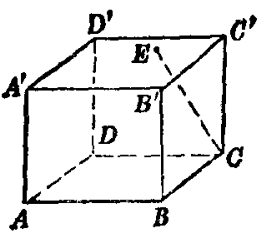
\includegraphics[width=4cm]{../pic/ltjh-ch1-xiti4-14.png}\\
    (第 14 题)
\end{minipage}

\end{xiaotis}

